\documentclass[11pt,letterpaper]{article}
\usepackage[margin=1in]{geometry}
\usepackage[T1]{fontenc}
\usepackage{tgpagella,microtype}
\usepackage{amsmath,amssymb,booktabs,tabularx,array,graphicx,xcolor}
\usepackage{enumitem,caption,placeins}
\usepackage[colorlinks=true,linkcolor=black,citecolor=black,urlcolor=blue!45!black,
 pdftitle={External Evidence and Language-Model Forecasts: A Blinded Comparison with Prediction-Market Prices},
 pdfauthor={Vorhersage}]{hyperref}
\hypersetup{bookmarksnumbered=true}
\setlength{\emergencystretch}{2em}
\setlength{\parskip}{3pt}
\captionsetup{font=small,labelfont=bf,labelsep=period}
\newcommand{\file}[1]{{\small\nolinkurl{#1}}}
\newcommand{\source}[2]{\href{#1}{#2}}
\newcolumntype{Y}{>{\raggedright\arraybackslash}X}
\newcommand{\ContractRows}{%
LAX high 74--75$^\circ$F (Sep.\ 18) & 3--4 & 3.5 & 12 & 5 \\
US unemployment $>4.4\%$ (Sep.) & 1--2 & 1.5 & 50 & 3 \\
Fed holds rates (Oct.\ 28) & 48--49 & 48.5 & 55 & 55 \\
Neutron launches before 2027 & 4--8 & 6 & 65 & 20 \\
Netflix film ranks first\textsuperscript{a} & 61--64 & 62.5 & 0.5 & 40 \\
Milwaukee beats Baltimore (Sep.\ 20) & 63--64 & 63.5 & 49 & 58 \\
}

\newcommand{\MetricRows}{%
Mean absolute gap & 33.17 & 8.58 & 27.75 \\
Root mean squared gap & 40.83 & 11.40 & 33.64 \\
Mean distance outside spread & 32.25 & 7.67 & 26.83 \\
}

\title{External Evidence and Language-Model Forecasts:\\
A Blinded Comparison with Prediction-Market Prices}
\author{}
\date{September 18, 2026}
\begin{document}
\maketitle
\begin{abstract}
We use prediction-market prices as prospective intermediate benchmarks for
evaluating language-model forecasts. Unresolved future events avoid leakage
of realized outcomes, while market prices provide immediate feedback from an
external, financially incentivized forecasting mechanism. Using the Vorhersage
workbench, we compare question-only and evidence-supplied forecasts for six
unresolved Kalshi contracts across six subject areas. The model, instructions,
and response schema are held fixed, with one independent call per contract
and condition. Opening quotes are withheld until forecasts are sealed, and
Kalshi is excluded as a source of research evidence. Mean absolute deviation
from the opening bid--ask midpoint is
33.17 percentage points in the question-only condition and 8.58 points in the
research condition. Research is associated with a smaller deviation in five
cases and an unchanged deviation in one. These results demonstrate improved
agreement with an economically meaningful intermediate benchmark. The small
purposive sample and single draw per condition limit generalization; a
documented entity-identification error also persists in the Netflix forecast.
The design supports rapid, reproducible comparisons before settlement, which
can subsequently be extended with outcome scoring.
\end{abstract}

\section{Introduction}
A forecasting system must translate evidence about an event into a numerical
probability. Liquid prediction markets provide a useful intermediate benchmark
for evaluating those probabilities before events resolve. This study asks
whether supplying current, relevant facts moves a model's forecasts closer to
that benchmark by comparing two
information conditions on the same set of unresolved prediction-market
contracts. One condition supplies only the event definition; the other adds a
frozen packet of primary-source evidence. Both use the same language model and
forecasting instructions.

There is a substantial empirical basis for this choice. Wolfers and Zitzewitz
\cite{wolfers2004} document accurate market forecasts across several settings
and favorable comparisons with conventional benchmarks. Page and Clemen
\cite{page2013} find reasonably well-calibrated probabilities for shorter-horizon
contracts, alongside horizon-dependent biases. In a distinct test of
forecasting accuracy, Berg, Nelson, and Rietz \cite{berg2008} find that Iowa
Electronic Markets vote-share forecasts are closer to eventual election
results than 74\% of 964 contemporaneous polls. The latter is evidence about
vote-share accuracy, rather than calibration of binary event probabilities.
Wolfers and Zitzewitz \cite{wolfers2006} also provide theoretical conditions
under which prices recover average beliefs, and show useful approximations
under broader assumptions. Together, this literature motivates well-traded,
clearly specified contracts as informative probability benchmarks, with
attention to liquidity and forecast horizon.

The prospective design has an additional advantage for evaluating language
models. For a genuinely unresolved future event, the eventual realized outcome
does not yet exist to be memorized in training data or retrieved from a later
account. Evaluating at that point avoids the realized-outcome leakage that can
affect historical forecasting exercises, without requiring reconstruction of
a historical information set. Market quotes make evaluation possible
immediately, rather than only after all events settle. Exposure to the market
price is a separate issue: this experiment withholds target quotes and excludes
market commentary from the forecasting inputs. The measured quantity is
\emph{market agreement}, interpreted as performance against an empirically
motivated intermediate probability benchmark.

Vorhersage provides the registration, evidence storage, forecast validation,
and separation of hidden targets from model inputs. The present experiment
uses a minimal direct-judgment method to isolate the information contrast as
far as possible. It does not compare the package's full structured workflow
with an unstructured alternative. The dated protocol, registration, and
result artifacts provide the empirical record for the analysis
\cite{protocol,results}.

\section{Experimental design}
\subsection{Contract selection and target measurement}
The sample consists of six contracts selected to span weather, employment,
monetary policy, space technology, entertainment, and sports. Candidate
contracts and ordered substitutes were recorded before order-book retrieval.
Previously revealed cases were excluded. Eligibility required an active,
unresolved binary contract; an uncrossed, non-extreme two-sided book; at least
one contract at each best quote; and a bid--ask spread no greater than ten
cents. Two initial candidates failed these requirements and were replaced by
predefined substitutes. The researcher received eligibility flags without
seeing accepted or rejected quotes. This procedure limits direct selection on
observed prices, although quote eligibility still conditions the sample. The
cohort was selected purposively rather than sampled randomly.

Opening books were captured on September 18, 2026, between 11:06:23 and
11:06:26 UTC (7:06 a.m.\ EDT), before external research. The reference value is
the arithmetic midpoint of the best YES bid and ask. Equal weight is assigned
to each contract, irrespective of quoted size, topic, or forecast horizon.
Table~\ref{tab:contracts} identifies the events and recorded probabilities.

\subsection{Information conditions and forecasting procedure}
An experimental \emph{arm} in Vorhersage binds a versioned method, model
configuration, and data assignment. Both arms used Google's
\texttt{gemini-3.1-pro-preview} with identical instructions and output schemas.
The question-only arm received the precise event and settlement conditions.
The research arm received those inputs plus a frozen packet containing source
excerpts, dates, extracted facts, and limitations. An external coding agent
selected and collected the evidence from official sources; the forecasting
model itself had no browsing tools or local filesystem access. Across the
six packets, nine source records were supplied. Appendix~\ref{app:evidence}
describes their contents and omissions.

Each contract received one fresh model call per arm, producing twelve
forecasts. Both arms were generated after evidence collection, in separate
contexts. Consequently, the question-only estimate is an information
ablation, not a chronological pre-research forecast. The common task requested
a probability, a concise rationale, reasons the estimate could be too high or
too low, and limitations. The method had an assessment stage followed by
deterministic issuance, with no model review or adjudication. Full settings
and execution details appear in Appendix~\ref{app:package}.

\subsection{Blinding and provenance}
\label{sec:blinding}
Kalshi supplied contract definitions and evaluator targets, but no Kalshi
material was used as research evidence. The package exposed only allowlisted
contract-definition fields to the researcher. Opening order books were saved
in a separate evaluator database; the research project stored commitments to
the hidden targets. Research was restricted to approved primary-source
domains. URL and redirect checks, together with lexical screening of returned
text, were applied before display to exclude prediction-market and
betting-odds material. Forecasting prompts contained only the assigned
question, common instructions, and permitted evidence.

All twelve forecasts were sealed at 11:25:10 UTC. Targets were revealed
between 11:40:25 and 11:40:27 UTC, after the study's reveal routine verified an
unchanged forecast seal and a terminal attempt for every registered trial.
The subsequent audit checked target commitments, evidence and forecast
hashes, and recorded timing \cite{audit}. The design provides auditable
procedural blinding: the exact hosted-model inputs are inspectable, although
the coordinator was not isolated from the evaluator database by operating
system permissions. Remaining leakage concerns involve market prices or
market-derived commentary, which lexical filters may not always detect.
These are distinct from leakage of the future realized outcome, which is
unavailable at the time of this prospective exercise.

\subsection{Evaluation measures}
Let $i=1,\ldots,n$ index contracts, with $n=6$, and let
$k\in\{Q,R\}$ denote the question-only and research conditions. Write $b_i$
and $a_i$ for the opening YES bid and ask, $q_i=(b_i+a_i)/2$ for their midpoint,
and $p_{ik}$ for the model forecast. The primary descriptive measure is mean
absolute deviation from the midpoint, expressed in percentage points:
\begin{equation}
 \mathrm{MAE}_k = \frac{100}{n}\sum_{i=1}^{n}|p_{ik}-q_i|.
 \label{eq:mae}
\end{equation}
We also report root mean squared deviation and mean distance outside the
opening bid--ask interval:
\begin{align}
 \mathrm{RMSE}_k &=100\sqrt{\frac{1}{n}\sum_{i=1}^{n}(p_{ik}-q_i)^2},\\
 \mathrm{Outside}_k &=\frac{100}{n}\sum_{i=1}^{n}
 \max\{b_i-p_{ik},\ p_{ik}-a_i,\ 0\}.
\end{align}
The paired improvement for contract $i$ is
$\Delta_i=100(|p_{iQ}-q_i|-|p_{iR}-q_i|)$; positive values indicate closer
agreement in the research arm. A constant forecast of 0.5 provides an
additional reference. The bid--ask interval describes quoted trading prices,
not a statistical confidence interval.

Squared distance from a probability benchmark has a direct scoring
interpretation. In the ideal case where $q_i=\mathbb{E}[Y_i\mid\mathcal{I}_i]$
is the event probability conditional on the relevant information set and
$p_{ik}$ is measurable with respect to that set,
\begin{equation}
\mathbb{E}\!\left[(p_{ik}-Y_i)^2-(q_i-Y_i)^2\mid\mathcal{I}_i\right]
= (p_{ik}-q_i)^2.
\end{equation}
Thus squared deviation equals expected excess Brier loss relative to that
ideal benchmark, without needing to observe the particular realization.
Market prices provide an empirically motivated proxy for this conditional
probability. The identity states the ideal-reference assumption explicitly;
marginal calibration alone does not establish it for each contract. The
current analysis measures the proxy directly, while subsequent settlement
permits a complementary outcome-based evaluation.

\section{Results}
\subsection{Aggregate and contract-level agreement}
Mean absolute deviation is 33.17 percentage points for question-only forecasts
and 8.58 points for research forecasts, a paired mean reduction of 24.58
points. Research yields closer agreement in five contracts and identical
agreement in the remaining contract (Figure~\ref{fig:performance}). No
contract was excluded after forecasting. All twelve responses passed
validation on their first attempt; none was repaired or rerun.

\begin{figure}[!htbp]
\centering
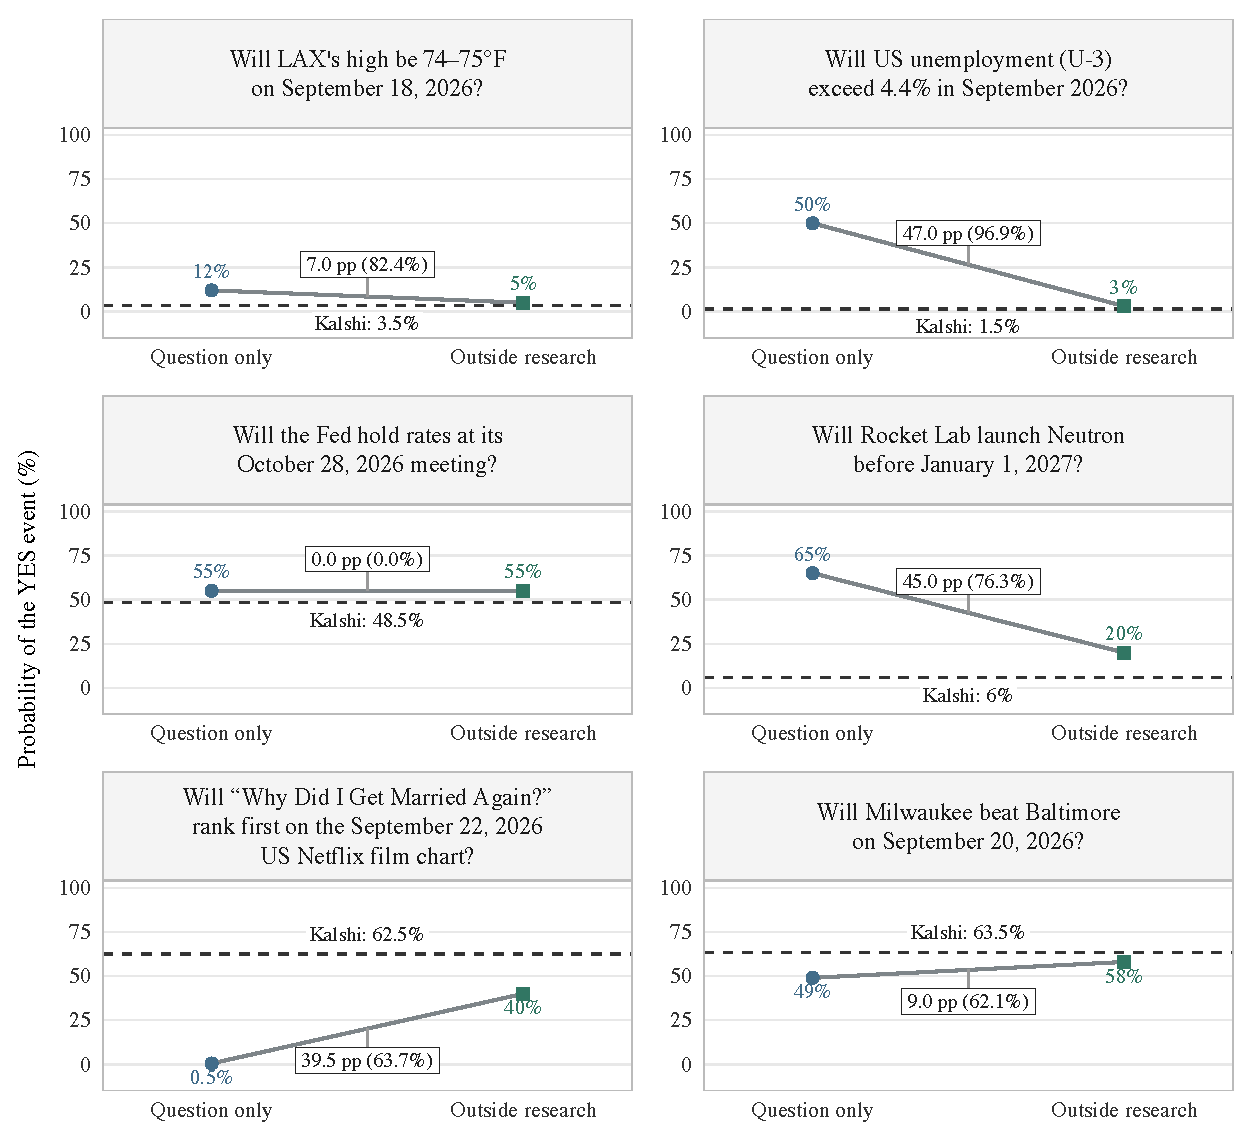
\includegraphics[width=\linewidth]{figures/performance.pdf}
\caption{\textbf{Forecast probabilities and opening Kalshi midpoints by question.}
Each panel connects the question-only forecast on the left to the
outside-research forecast on the right. A labeled horizontal dashed line marks
the opening Kalshi midpoint. The vertical distance from each forecast to this
line is its absolute market deviation. Boxed slope labels report the reduction
in that deviation in percentage points and, in parentheses, as a percentage of
the question-only deviation: $100(d_Q-d_R)/d_Q$, where $d_k=|p_k-q|$.
Positive values indicate improvement. Endpoint labels report probabilities;
all panels share a 0--100\% scale. The two forecasts are separate information
conditions, not chronological updates.}
\label{fig:performance}
\end{figure}

The constant-50\% reference has a mean absolute deviation of 27.75 points,
falling between the two model conditions. Research also has lower root mean
squared deviation (11.40 versus 40.83 points) and lower mean distance outside
the opening spread (7.67 versus 32.25 points). Table~\ref{tab:metrics} reports
all three measures on the same six-contract cohort. Follow-up quotes collected
at reveal have unchanged midpoints for every contract, so the midpoint-based
results are identical using those later observations. Netflix's spread
widens from three to seven cents.

\begin{table}[!htbp]
\centering\small
\caption{Contract definitions and probabilities.}
\label{tab:contracts}
\setlength{\tabcolsep}{4pt}\renewcommand{\arraystretch}{1.15}
\begin{tabularx}{\linewidth}{Yrrrr}
\toprule
& \multicolumn{2}{c}{Opening market (\%)} & \multicolumn{2}{c}{Forecast (\%)}\\
\cmidrule(lr){2-3}\cmidrule(l){4-5}
YES event & Bid--ask & Midpoint & Question only & Research\\
\midrule
\ContractRows
\bottomrule
\end{tabularx}
\par\vspace{4pt}
\begin{minipage}{\linewidth}\footnotesize
\emph{Notes:} All dates are in 2026.
\textsuperscript{a}\emph{Why Did I Get Married Again?} ranks first in the US
Netflix film chart published September 22 for the week ending September 20.
The contract headline refers to September 21; settlement rules define the event.
\end{minipage}
\end{table}

\begin{table}[!htbp]
\centering\small
\caption{Deviation from the opening market benchmark.}
\label{tab:metrics}
\renewcommand{\arraystretch}{1.15}
\begin{tabularx}{\linewidth}{Yrrr}
\toprule
Measure (percentage points) & Question only & Research & Constant 50\%\\
\midrule
\MetricRows
\bottomrule
\end{tabularx}
\par\vspace{4pt}
\begin{minipage}{\linewidth}\footnotesize
\emph{Notes:} Equal-weight averages over all six contracts, using the opening
midpoint as an intermediate probability benchmark. The constant-50\% condition
is computed mechanically and requires no additional model calls.
\end{minipage}
\end{table}

\FloatBarrier
\subsection{Evidence use and observed failure modes}
The largest reductions in absolute deviation occur for unemployment (47
points), Neutron (45 points), and Netflix (39.5 points). For unemployment,
the BLS reading of 4.1\% provides a current anchor: the contract's strict
threshold requires a published rate of at least 4.5\%. The forecast falls
from 50\% to 3\%. For Neutron, the company update concerns Q4 delivery to the
launch pad, rather than a guaranteed launch that quarter. The forecast falls
from 65\% to 20\%, but remains fourteen points above the market midpoint.

The Netflix case illustrates a limitation of both source selection and model
interpretation. Both responses reason as though the target were an older
catalog film. Official discovery identified a September 2026 release, but
the packet preserved the previous week's number-one ranking without the
release date. This omission and the entity-identification error were recorded
at 11:25:43 UTC, before target reveal \cite{audit}. The original forecasts
remain in the analysis: research raises the estimate from 0.5\% to 40\%,
compared with a midpoint of 62.5\%.

Smaller reductions occur for Milwaukee baseball (nine points) and LAX
weather (seven points). Team records and run differentials favor Milwaukee,
but the packet lacks starting pitchers, lineups, and bullpen context. For
LAX, an NWS forecast high of 79$^\circ$F lies outside the 74--75$^\circ$F event
interval, reducing the forecast from 12\% to 5\%. The probability assigned to
that interval is not supported by an estimated forecast-error distribution.
Finally, both Fed forecasts are 55\%, despite the researched explanation
incorporating the latest policy decision and year-end projections. Equal
probabilities therefore do not imply equal factual grounding.
\FloatBarrier

\section{Discussion}
The results show a substantial improvement against the market benchmark:
research reduces the mean absolute gap by 24.58 percentage points and improves
agreement in five of six cases. Given the forecasting and calibration evidence
for prediction markets, this is a useful intermediate performance result.
The design produces feedback while outcomes remain in the future, permitting
research methods to be compared without waiting for settlement or introducing
realized-outcome leakage through retrospective data collection.

The relevant experimental contrast is access to current evidence. The
question-only condition lacks fresh facts that are directly relevant to
several events, so a subsequent comparison can distinguish a minimal factual
update from deeper, adaptive research. Review, scenario modeling, and
ensembles remain additional dimensions to test. Source collection here was
performed by an external coding agent; the results concern that research
pipeline coupled to the forecasting model.

Several additional limitations matter. First, six purposively selected
contracts do not support a population-level performance estimate. Employment
and monetary policy are related, and contract horizons differ substantially.
Second, one draw per condition leaves model sampling variability unmeasured;
the observed paired differences combine information-condition differences
with stochastic generation. We report no significance test or inferential
interval. Third, the strongest case for a price benchmark concerns liquid,
well-functioning markets. This pilot's minimal two-sided-quote requirement
does not establish deep liquidity: Neutron's opening best bid has a size of
only five contracts. Larger studies should prespecify stronger depth and
spread criteria and examine performance by horizon, reflecting the empirical
calibration evidence \cite{page2013}. Fourth,
research follows the opening snapshots. Unchanged follow-up midpoints reduce
concern about observed price movement during the run but do not establish
identical information sets. The remaining blinding limitations concern price
exposure, as described in Section~\ref{sec:blinding}.

The pilot also identifies a concrete design improvement: both information
conditions in a subsequent research-depth comparison should include verified
entity identities and relevant release or publication dates. A fresh,
unrevealed cohort could then compare a small current-facts packet with
additional targeted research, using repeated forecasts and registered
handling of failed submissions. Larger cohorts would permit paired
uncertainty estimates that account for related event groups. Retaining these
forecasts through settlement would add outcome scores and calibration checks
to the immediate market-based evaluation. These two forms of assessment are
complementary: prices support timely development and comparison, while
realizations allow the intermediate benchmark and the model forecasts to be
evaluated over repeated events.

\begin{thebibliography}{9}
\small
\bibitem{wolfers2004} Wolfers, J., and Zitzewitz, E. (2004).
Prediction markets. \emph{Journal of Economic Perspectives}, 18(2), 107--126.
\href{https://doi.org/10.1257/0895330041371321}{doi:10.1257/0895330041371321}.
\bibitem{page2013} Page, L., and Clemen, R. T. (2013).
Do prediction markets produce well-calibrated probability forecasts?
\emph{The Economic Journal}, 123(568), 491--513.
\href{https://doi.org/10.1111/j.1468-0297.2012.02561.x}{doi:10.1111/j.1468-0297.2012.02561.x}.
\bibitem{berg2008} Berg, J. E., Nelson, F. D., and Rietz, T. A. (2008).
Prediction market accuracy in the long run. \emph{International Journal of
Forecasting}, 24(2), 285--300.
\href{https://doi.org/10.1016/j.ijforecast.2008.03.007}{doi:10.1016/j.ijforecast.2008.03.007}.
\bibitem{wolfers2006} Wolfers, J., and Zitzewitz, E. (2006).
Interpreting prediction market prices as probabilities.
\emph{NBER Working Paper} 12200.
\href{https://doi.org/10.3386/w12200}{doi:10.3386/w12200}.
\bibitem{protocol} Study protocol and experimental registration (2026).
Vorhersage blinded Kalshi pilot, September 18.
\file{protocol.json}, \file{run/selection.json}, and \file{run/registration.json}.
\bibitem{results} Forecasts and market comparison (2026).
Vorhersage blinded Kalshi pilot, September 18.
\file{run/comparison.json}, \file{run/raw-records.json}, and
\file{run/revealed-targets/}.
\bibitem{audit} Integrity audit and pre-reveal diagnostics (2026).
Vorhersage blinded Kalshi pilot, September 18.
\file{run/audit.json} and \file{run/pre-reveal-diagnostics.json}.
\end{thebibliography}
\clearpage
\appendix
\section{Package architecture and execution}
\label{app:package}
Vorhersage 0.3.0 is a Python forecasting workbench with a command-line interface,
requiring Python 3.11 or later and no declared runtime dependencies. It preserves
questions, evidence, model inputs, forecasts, and evaluation records. The
external agent chooses sources and makes judgments; deterministic package code
checks schemas, bookkeeping, and declared numerical calculations. Stored
provenance makes a claim inspectable but does not establish that it is true.

\subsection{Components and responsibilities}
\small
\renewcommand{\arraystretch}{1.16}
\begin{tabularx}{\linewidth}{@{}p{1.57in}Y@{}}
\toprule
Component & Role in this study\\
\midrule
\file{store.py}, \file{schemas.py} & SQLite transactions, versioned questions,
immutable artifact records, content hashes, and validated submissions preserve
what each trial received and produced.\\
\file{experiments.py} & Registers a versioned method and separate arms binding
method, model configuration, and question-specific evidence. Freezes the cohort,
cutoffs, repetitions, and trial order.\\
\file{evidence.py} & Stores source captures, URLs, timestamps, excerpts, facts,
and limitations in packets linked to the assigned arm.\\
\file{workflow.py} & Advances each trial through assessment and issuance;
validates the submitted probability and rationale, then records the forecast.\\
\file{market_data.py} & Separates price-free contract definitions from private
quote snapshots; derives the YES ask from the complementary NO bid.\\
\file{workbench.py} & Keeps targets in a separate evaluator project, stores
commitments, and requires completion before reveal.\\
Study scripts & \file{study.py} coordinates selection, source filtering,
registration, import, forecast sealing, reveal, and audit.
\file{build_evidence.py} records the source-to-packet extraction.\\
\bottomrule
\end{tabularx}
\normalsize

\subsection{Arm specification and model configuration}
The shared method, \file{outside-source-direct-judgment}, uses only
\file{assessment} and \file{issue}. Assessment asks for a probability, concise
rationale, reasons it could be too high or too low, and limitations. Issuance
records the result; it is not another model call. The question-only arm assigns
no research packet, while the outside-research arm assigns its question's frozen
packet. Changing a registered method or arm requires a new version.

Both arms used temperature 0.5, topK 40, topP 1, maxOutputTokens 8192, and
thinking\_budget 2048. The model was called through an external EDSL transport
with tools disabled. This transport and the report's plotting dependencies are
separate from the dependency-free core. Prompts, provider records, raw answers,
accepted submissions, and issued forecasts were all retained. Model identity
and settings are those recorded by the transport, not an attestation about the
provider's internal implementation.

\subsection{Scope of the evaluated implementation}
The package also supports scenario mixtures, grouped likelihood-ratio updates,
timeline models, reference-class priors, review stages, ensembles, and scoring
against resolved outcomes. Those features were not used to produce these twelve
forecasts. Exa and Firecrawl adapters can preserve research-provider receipts,
but this run used browser tools and direct official HTTP requests because their
API keys were not configured. Thus the result concerns a frozen-evidence,
direct-judgment comparison, not the performance of every available workflow.

\subsection{Integrity checks and recorded costs}
The live audit verified all twelve issued forecasts and six opening-target
commitments, with 82 artifacts passing database integrity checks. Fourteen
focused tests covered source restrictions, quoted-odds rejection, premature or
tampered reveal prevention, and metric arithmetic. All twelve model responses
were accepted on their first attempt. Summed provider-reported model cost was
\$0.16835. Research, browser, and coordinator dollar costs are unknown,
not zero; this number is not total system cost. The ledger records fourteen
direct HTTP attempts (seven successful), six browser searches, and six browser
page-read operations across five tool calls.

\section{Evidence and reproducibility}
\label{app:evidence}
\subsection{The six frozen evidence packets}
The packets contain nine source records. The following links identify the
original sources; the dated captures in the run are authoritative for what the
model received, since live pages may subsequently change.

\begin{description}[leftmargin=0pt,labelsep=.5em,itemsep=3pt,font=\normalfont\itshape]
\item[Weather.]
\source{https://api.weather.gov/gridpoints/LOX/148,41/forecast}{NWS point forecast}
and the
\source{https://forecast.weather.gov/product.php?site=LOX\&issuedby=LAX\&product=CLI\&format=CI\&version=1\&glossary=1}{LAX climate report}:
forecast high 79$^\circ$F, previous high 78$^\circ$F, and normal high 76$^\circ$F.
The packet does not estimate forecast errors and uses NWS as a proxy for the
contract's commercial settlement source.
\item[Employment.]
\source{https://www.bls.gov/news.release/archives/empsit_09042026.htm}{BLS employment report, September 4}:
August and July unemployment 4.1\%, June 4.2\%, and August payroll growth
162,000. The September report was scheduled for October 2. The contract's
strict threshold requires a published rate of at least 4.5\%.
\item[Monetary policy.]
\source{https://www.federalreserve.gov/newsevents/pressreleases/monetary20260916a.htm}{September 16 FOMC statement}
and
\source{https://www.federalreserve.gov/monetarypolicy/fomcprojtabl20260916.htm}{economic projections}:
a 25-basis-point hike to 3.75--4.00\%, unanimous 12--0 vote, and a median year-end
rate projection of 4.1\%. Year-end projections do not identify the meeting at
which a subsequent change occurs.
\item[Space technology.]
\source{https://investors.rocketlabcorp.com/news-releases/news-release-details/rocket-lab-announces-second-quarter-2026-financial-results-posts}{Rocket Lab second-quarter update, August 10}:
first-flight assembly and testing, with first-stage tank delivery to the pad
aligned to Q4. The issuer's forward-looking update lacks a complete remaining
test and launch-readiness schedule.
\item[Entertainment.]
\source{https://www.netflix.com/tudum/top10/united-states}{Netflix US film chart}:
the target title ranked first for September 7--13. Its
\source{https://www.netflix.com/tudum/articles/tyler-perrys-why-did-i-get-married-again?inapp=true}{September 9 release date}
was found during discovery but omitted from the model's packet. The error was
logged in \file{run/pre-reveal-diagnostics.json} at 11:25:43 UTC.
\item[Sports.]
\source{https://statsapi.mlb.com/api/v1/schedule?sportId=1\&date=2026-09-20\&teamId=158\&hydrate=probablePitcher,team}{MLB schedule}
and
\source{https://statsapi.mlb.com/api/v1/standings?leagueId=103,104\&season=2026\&date=2026-09-17\&standingsTypes=regularSeason}{standings}:
Milwaukee at Baltimore on September 20; records of 95--58 and 75--78, with run
differentials of $+197$ and $-26$. No usable starting-pitcher, lineup, injury,
or bullpen context entered the packet.
\end{description}

\subsection{Research artifacts and reproducibility}
Paths are relative to \file{examples/kalshi_blind_20260918/}. The protocol and
candidate order preceded price inspection; experiment registration followed
evidence collection at 11:19:02 UTC.

\small\renewcommand{\arraystretch}{1.13}
\noindent
\begin{tabularx}{\linewidth}{@{}>{\raggedright\arraybackslash}p{2.35in}Y@{}}
\toprule
Record & What it establishes\\
\midrule
\file{protocol.json}; \file{run/selection.json} & Planned comparison, source rules, and ordered candidates.\\
\file{run/registration.json}; \file{run/*-arm.json} & Frozen questions, method/model/data assignments, and trials.\\
\file{run/packets/}; \file{run/tasks/} & Exact evidence and prompts available to each call.\\
\file{run/raw-records.json}; \file{run/attempts.json} & Responses, attempt outcomes, and model costs.\\
\file{run/sealed-forecasts.json}; \file{run/audit.json} & Forecast seal, hash checks, and timing.\\
\file{run/comparison.json}; \file{run/revealed-targets/} & Numerical results and original revealed target receipts.\\
\bottomrule
\end{tabularx}\normalsize

\file{plot_performance.py} recomputes all three aggregate metrics for all three
conditions and verifies them against the frozen comparison before generating
the table rows and calling \file{plot_performance.R} for the faceted slope graph.
The R script also verifies the metrics and renders the figure using ggplot2.
With Python, R (ggplot2 3.5.0 or later and jsonlite), and LaTeX available,
run from this study directory:
\begin{quote}\small\ttfamily
python plot\_performance.py\\
latexmk -pdf -interaction=nonstopmode -halt-on-error report.tex
\end{quote}
Rebuilding makes no model or market calls. A new blind experiment requires
unrevealed contracts and a separate directory preserving the registration,
sealing, and reveal order.
\end{document}
